\section{Pulsar Magnetosphere}

The basic picture of a pulsar magnetosphere was first presented in
\cite{goldreich_1969_pulsar-electrodynamics}.  The magnetic dipole
of the rotating \ac{NS} creates a quadrupole electric field.
The component of the electric field along the open field lines acts as
a powerful particle accelerator which can extract and accelerate charged
particles from the \ac{NS}. The potential generated
by this field is given as \citep{goldreich_1969_pulsar-electrodynamics}:
\begin{equation}
\PulsarPotential = \frac{\MagneticField \angularfrequency^2 \PulsarRadius^2}{2c^2}
\approx 6\times 10^{12} 
\left(\frac{\MagneticField}{10^{12}\unitspace\gauss}\right)
\left(\frac{\PulsarRadius}{10\unitspace\km}\right)^3
\left(\frac{\period}{1\unitspace\second}\right).
\end{equation}

\figref{pulsar_magnetosphere} shows a schematic diagram of this
magnetosphere.


\begin{figure}[htpb]
  \begin{center}
    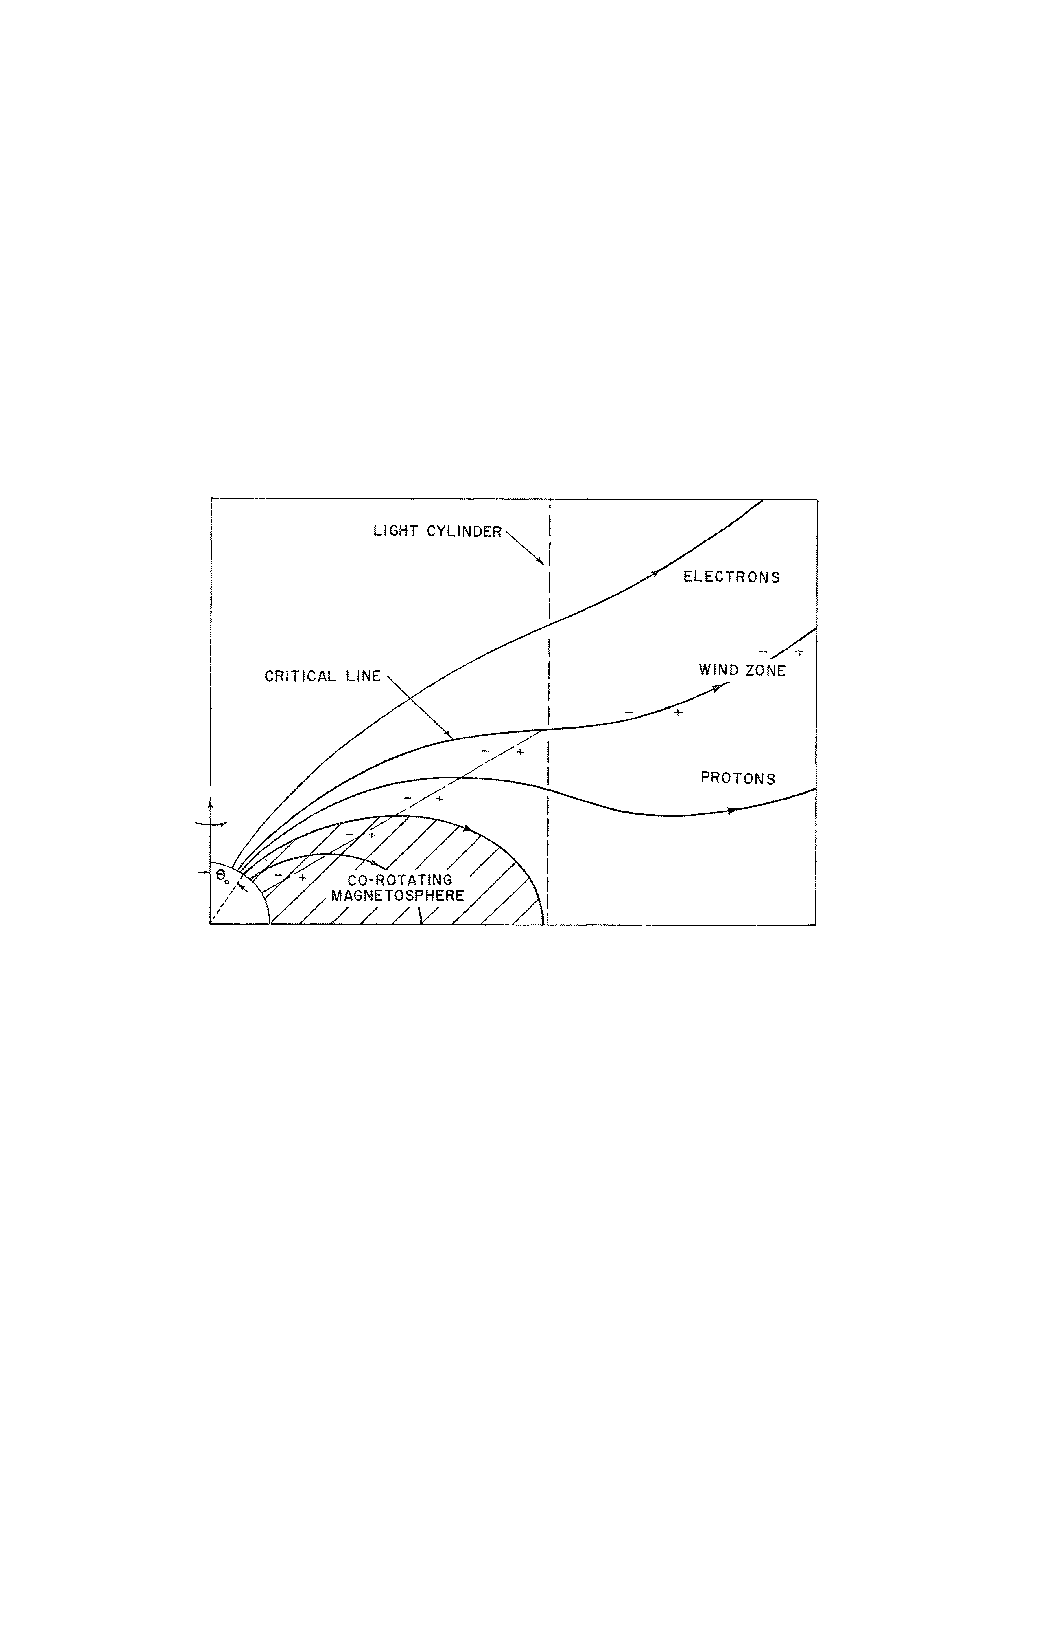
\includegraphics{chapters/pulsar_pwn_system/figures/pulsar_magnetosphere.pdf}
  \end{center}
  \caption{The magnetosphere for a rotating pulsar.
  The pulsar is on the bottom left of the plot. This figure is
  from \cite{goldreich_1969_pulsar-electrodynamics}.}
  \figlabel{pulsar_magnetosphere}
\end{figure}



Pulsars typically release a small amount of their overall energy
budget as pulsed emission. The efficiency of converting
spin-down energy inot pulsed $\gamma-$rays is typically
$\sim$ 0.1\% to 10\% (\cite{abdo_2010a_first-fermi}).
For example, the Crab nebulae is estimated to release 0.1\%
of it's spin-down energy as pulsed $\gamma$-rays \cite{abdo_2010a_fermi-large}.
The energy released as radio and optical photons is typically much less.
For the crab,

Of the energy released during this process, only a very small fraction of the 
radiation is released in radio. For example, 
for the Crab pulsar, the $\gamma$-ray efficiency of 


\begin{itemize}
\item "While the pulsars emit in the radio band a tiny <= $10^{-6}$
fraction of their rotational energy (Manchester \& Taylor 1977), the
γ-ray luminosities of some of the EGRET pulsars above 100 MeV exceed
one per cent of their spin-down luminosities." -- aharonian\_2003\_exploring-physics
  \item What fraction is released in PWNe?
\end{itemize}

Crab nebulae flux:

radio 6e-14
optical: 8e-12
x-ray 1.5e-9 -- fritz\_1969\_x-ray-pulsar erg cm\^-2 sec\^-1
gamma-ray, efficiency=0.001, flux=1.3e-9 erg cm\^-2, sec\^-1  \url{http://arxiv.org/pdf/0910.1608v4.pdf}



Energetics of PWNe:

``The efficiency of conversion of spin-down luminosity into synchrotron
emission is defined by efficiency factors η and
η LX/E  Typical values are η
and η (Becker \& Trumper 1997, Frail
\& Scharringhausen 1997), although wide excur- sions from this are
observed. Note that if the synchrotron lifetime of emitting particles is
a significant fraction of the PWN age (as is almost always the case at
radio wavelengths, and sometimes also in X-rays), then the PWN emission
represents an integrated history of the pulsas spin down,
and ηR and ηX are not true instantaneous efficiency factor'' --gaensler\_2006\_evolution-structure

X-ray energetics tabulated from: \url{http://arxiv.org/pdf/astro-ph/0006030v1.pdf}
